\documentclass[conference]{IEEEtran}  % US letter, the IEEE default
% IEEE conference template (IEEEtran 1.8b), chosen on 2026-10-26; the course left the template free.
% Built with pdfLaTeX, as IEEE builds it: latexmk -pdf main.tex
\usepackage{cite}  % numbered citations in brackets, sorted and compressed: [1], [3]-[5]
\usepackage{harmony}  % note values in the tables (\Vier, \Acht, ...), drawn with the MusiXTeX fonts
\usepackage{xcolor}  % grey for the draft's todos and the shaded table cells
% Package for lorem ipsum
\usepackage{lipsum}
\usepackage{graphicx}
\graphicspath{{../figures/}}  % written by the notebooks, shared with the slides
\usepackage[caption=false,font=footnotesize]{subfig}  % panels (a), (b), (c) under one caption, as IEEEtran's documentation recommends
\usepackage{colortbl}  % shaded cells in tables
\usepackage{fontawesome5}  % the GitHub logo by the repository link: its glyphs sit on the text baseline
\newcommand{\todo}[1]{{\color{gray}\itshape [#1]}}  % what the draft still lacks
\newcommand{\placeholder}[2][1-2]{{\itshape\lipsum[#2][#1]}}  % dummy text where a section is still to be written
% Package to link references, loaded last
\usepackage[hidelinks]{hyperref}  % links clickable but black, as in IEEE papers

\begin{document}
\title{Higher-Order Interactions in Musical Style:\\ Imitating Bach's Chorales and Palestrina's Masses\\ with Random Walks on Hypergraphs}
\author{\IEEEauthorblockN{Francesco Secoli}
\IEEEauthorblockA{Advanced Laboratory of Complex Network Analysis\\
University of Pisa, MSc in Data Science and Business Informatics\\
Pisa, Italy\\
\href{https://github.com/sclfnc/hypergraph-walks-bach-palestrina}{\faGithub\ GitHub repository}}}
\maketitle

\begin{abstract}
% TODO Written last, 150 to 250 words, in this order: context, gap, research question and hypothesis, data and network model, method with the null model, main result with a number, what it implies.
% Draft of 2026-10-26: the parts that do not exist yet are marked with \todo.
A model that imitates a musical style has to reproduce rules that bind several voices at once, such as the ban on consecutive fifths. Statistical models of four-part harmony count either pairs of notes, which miss these rules, or whole sonorities, which recur too rarely to cover new music. The configurations in between are what network science calls higher-order interactions, and in the sources we checked no model counts them in a corpus to generate music. We ask whether a random walk on a hypergraph can imitate a musical style, and which parts of the hypergraph it needs. \todo{the hypothesis, once H0 and H1 are fixed} For 352 chorales by Bach and 1,179 movements of Palestrina's masses, set on a common time grid and key, the hyperedges are configurations of a few voices over a few cells, each weighted by its support in the corpus. The walk writes the lower voices under a given melody from these counts alone. Removing one shape of hyperedge at a time, and testing on tunes and masses that the counts have not seen, shows which shapes the imitation needs. \todo{the null model; the main result, with its number; what it implies}

\end{abstract}

\begin{IEEEkeywords}
Bach chorales, higher-order interactions, hypergraphs, music generation, Palestrina, random walks
\end{IEEEkeywords}

\section{Introduction}
% Un po' debole su Palestrina, da rafforzare
% Draft of 2026-10-26, kept general on purpose. Works marked [S] or [A] in bib/literature_search_2026-10-15.md (search summary or abstract only) are cited here for general statements; read them before any precise claim.

% Migliorare la narrazione: 

Algorithmic composition has used grammars, rule systems, evolutionary search, Markov chains and neural networks \cite{fernandez2013, herremans2017}, and the methods that learn from a corpus are used primarily to imitate a style \cite{fernandez2013}. The four-part harmonisation of Bach's chorales is a common test of this imitation. Expert systems write the rules of the style by hand \cite{ebcioglu1988}, statistical models count it in a corpus \cite{allan2004, whorley2016, zhu2021}, and neural networks learn it \cite{hild1991, hadjeres2017, liang2017, huang2017}. 
% semplificare e dichiarare risultati contrastanti in letteratura con una citazione unificante
The families do not agree on what a better harmonisation is: one comparison favours the rule-based system \cite{phonamnuaisuk1999}, another finds the stochastic methods more interesting and less correct \cite{sikora2023}.

Statistical models of the task count pairs of notes or whole sonorities, while the rules of counterpoint bind a few voices over a few moments: what network science calls higher-order interactions \cite{battiston2020}. 
% Introdurre meglio e giustificare meglio l'esplorazione, discutendone con l'utente.
We ask whether a hypergraph walk can imitate a musical style, and which parts it needs. For two styles, Bach's chorales and Palestrina's masses, we build a hypergraph whose hyperedges are configurations of a few voices over a few moments, weighted by how often they occur, and a random walk on it writes the lower voices under a given melody. Removing one kind of hyperedge at a time shows which parts the imitation needs. The contributions are three:
% TODO check each contribution against the results before the final version.
\begin{itemize}
\item a hypergraph of a polyphonic corpus whose hyperedges are the configurations on which rules of style are defined, each weighted by its support;
\item a generation by random walk that uses only these counts, with no learned parameter;
\item an ablation of the hyperedge shapes on two styles, more than a century apart.
\end{itemize}

\subsection{Related Work}

The statistical models differ in what they count. Some count the change from one whole sonority to the next \cite{allan2004, whorley2013}; others count pairs of notes, across voices and across time \cite{hadjeres2016}. Pairs miss the rules that bind two voices over two moments: a pairwise model reproduces many of these configurations, yet writes consecutive fifths and octaves far more often than Bach \cite{hadjeres2016}. Whole sonorities, at the other end, recur too rarely to cover new music. The rules of counterpoint live in between, on a few voices over a few moments \cite{fux1725}.

Network science has a language for these intermediate configurations: higher-order interactions, which join more than two nodes at once \cite{battiston2020}, with their own motifs and null models \cite{lotito2022}. Music has been read as a network of notes or chords linked in pairs \cite{kulkarni2024, dimarco2026}, and such networks have been walked to generate music \cite{liu2009}. Higher-order structures of music exist too: simplicial complexes of chords \cite{bigo2015, mrad2026} and hypergraphs whose hyperedges are the notes that sound together \cite{coupette2023}. They describe music, or transform a given piece \cite{bigo2015}. In the sources we checked, no model counts the higher-order configurations of a corpus and generates new music by walking on them.

\subsection{Organisation of This Work}

Section~\ref{sec:dataset} describes the two corpora and how we filter and label them, and Section~\ref{sec:representation} turns them into hypergraphs. The hypotheses and the method of the test follow in Section~\ref{sec:method}, the results in Section~\ref{sec:results}, and the conclusions in Section~\ref{sec:conclusions}.

\section{Dataset}
\label{sec:dataset}
The study uses 352 Bach chorales and 1,179 movements of Palestrina's masses, selected from the music21 corpus \cite{cuthbert2010} by six successive filters that make the data uniform.
\subsection{Sources}

Both corpora are distributed with music21 \cite{cuthbert2010, cuthbert2026music21}. The Bach corpus holds 413 files, nearly all chorales: Lutheran hymn tunes that Bach set for four voices. The Palestrina corpus holds 1,318 files, each a movement of a mass or a section of one, which John Miller encoded from the modern complete edition \cite{palestrina1939}.

The scores hold no personal data, so the General Data Protection Regulation does not apply. The copyrights of the Palestrina files and of three Bach files reserve the rights to derivative electronic formats, so the repository holds code only (Section~\ref{sec:availability}).

\begin{table}[t]
\renewcommand{\arraystretch}{1.3}
\centering
\caption{Files and notes removed by each filter, in order.}
\label{tab:filters}
\begin{tabular}{@{}lcccc@{}}
\hline
& \multicolumn{2}{c}{Bach} & \multicolumn{2}{c}{Palestrina} \\
\cline{2-3} \cline{4-5}
& files & notes & files & notes \\
\hline
Raw dump & 413 & 112,010 & 1,318 & 717,031 \\
\emph{Removed by} & & & & \\
\quad meter & 51 & 16,071 & 115 & 25,832 \\
\quad not a chorale & 1 & 598 & -- & -- \\
\quad voices & 1 & 10,122 & -- & -- \\
\quad bars & 6 & 1,690 & -- & -- \\
\quad copies & 2 & 702 & 21 & 11,419 \\
\quad off the grid & -- & -- & 3 & 1,726 \\
\hline
Kept & 352 & 82,827 & 1,179 & 678,054 \\
\quad share kept (\%) & 85.2 & 73.9 & 89.5 & 94.6 \\
\hline
\end{tabular}
\end{table}

\subsection{Cleaning and Filtering}

We filter both corpora so that one representation fits every piece: the same bar of four beats, the same time grid, and only the sung voices. This uniformity makes different pieces comparable and keeps the representation simple. Table~\ref{tab:filters} counts what each filter removes, in the order in which we apply them; the meter filter removes the most notes.

\subsubsection{Meter}
A single bar of four beats gives every piece the same pattern of strong and weak beats, and one time grid that fits them all. A piece therefore stays only if it keeps a bar of four beats from start to end: 4/4 in Bach, where the beat is a quarter note, and 4/2 in Palestrina, where the beat is a half note. This filter removes mostly pieces in triple meter, with three beats to the bar, and the few pieces whose time signature changes along the way.

\subsubsection{Not a chorale}
A Bach file stays only if it is a chorale. This filter removes the one file that is not: BWV 846, the first prelude of the Well-Tempered Clavier, a keyboard piece on two staves.

\begin{table}[t]
\renewcommand{\arraystretch}{1.3}
\centering
\caption{Files and notes on the grid, per grid step in the raw dump; shaded: chosen step.}
\label{tab:grid}
\begin{tabular}{@{}clcccc}  % note symbols smashed: the flags would make their rows taller
\hline
& & \multicolumn{2}{c}{Bach (\%)} & \multicolumn{2}{c}{Palestrina (\%)} \\
\cline{3-4} \cline{5-6}
\multicolumn{2}{@{}l}{Grid step} & files & notes & files & notes \\
\hline
\smash{\raisebox{-0.3ex}{\scalebox{0.72}{\Zwdr}}} & thirty-second & 100.00 & 100.00 & 99.77 & 99.96 \\
\smash{\raisebox{-0.3ex}{\scalebox{0.72}{\Sech}}} & sixteenth & \cellcolor{gray!18}98.06 & \cellcolor{gray!18}99.96 & 99.77 & 99.96 \\
\smash{\raisebox{-0.3ex}{\scalebox{0.72}{\Acht}}} & eighth & 30.99 & 97.07 & \cellcolor{gray!18}99.77 & \cellcolor{gray!18}99.96 \\
\smash{\raisebox{-0.3ex}{\scalebox{0.72}{\Vier}}} & quarter & 1.21 & 76.46 & 19.73 & 99.32 \\
\smash{\raisebox{-0.3ex}{\scalebox{0.72}{\Halb}}} & half & 0.00 & 38.76 & 0.23 & 86.31 \\
\smash{\raisebox{0.3ex}{\scalebox{0.72}{\Ganz}}} & whole & 0.00 & 20.65 & 0.00 & 52.74 \\
\hline
\end{tabular}
\end{table}

\subsubsection{Voices}
A Bach chorale keeps only its four sung voices, Soprano, Alto, Tenor and Bass: the instrumental parts of a cantata occur in only 32 chorales, and keeping them would give these chorales a texture that the others lack. This filter removes these parts, and the 32 chorales stay with their four voices. It removes one chorale whole, BWV 227.3, which has five sung voices with two sopranos: reducing it to four would drop a sung line. A Palestrina movement keeps all its voices, from three to eight, because one mass mixes movements for different numbers of voices: only 450 of the 1,203 movements have exactly four. Its voices take the same four types and a fifth, Baritone, and a type that occurs twice is numbered, as in Tenor~1 and Tenor~2. In both corpora a voice is the line written in its part, also where two voices cross.

\subsubsection{Bars}
The pattern of strong and weak beats holds only if the downbeats stay four beats apart, from the first full bar to the last. In Bach, 266 chorales open with an upbeat and 206 split a bar in two, at a repeat sign or at the end of a phrase; these partial bars do no harm when their two pieces add up to four beats. In six chorales one bar has another length or lacks its other half, so every later downbeat falls on the wrong beat. This filter removes these six chorales whole: cutting out the irregular bar would remove music that Bach wrote. Palestrina's movements have neither upbeats nor split bars.

\subsubsection{Copies}
Comparing the files note by note, in any key, we remove one file of each identical pair; the check finds all six duplicates listed by Dahn \cite{dahn2018} that the corpus contains. Twenty pieces remain in more than one version, differing by at most 7.4\% of their notes; Section~\ref{sec:transformations} weights them.

\subsubsection{Off the grid}
This filter anticipates the model of Section~\ref{sec:transformations}, which reads time on a grid of equal cells. The coarsest grid that keeps 99.9\% of the notes of the raw dump is a quarter of the beat: a sixteenth note in Bach and an eighth note in Palestrina (Table~\ref{tab:grid}). In Bach, nine thirty-second notes of a written-out ornament fall between grid lines, and Section~\ref{sec:transformations} shows how the grid keeps them. In Palestrina, three movements hold triplet minims, which the grid would turn into a duple rhythm that Palestrina did not write; this filter removes these movements whole, so that the corpus holds pieces instead of fragments.

\subsection{Keys and Tonal Types}
\label{sec:keys}

To move every piece to a common key (Section~\ref{sec:transformations}), we label each chorale with its key and each Palestrina movement with its tonal type.

Of the 352 chorales, 304 take their key from an expert analysis of the When in Rome corpus \cite{gotham2023, gotham2026wir}, matched on the file name. The other 48 take their key from a fixed rule that combines five key profiles with the key signature. A Palestrina movement takes its tonal type in the sense of Powers \cite{powers1981}: the system, \emph{cantus durus} or \emph{cantus mollis} (no flat or one flat in the signature), and the final, the lowest note of the closing sonority. Powers adds a third marker, the cleffing, which the modern clefs of the files do not keep. The label names no mode, because a tonal type can stand for a mode without being that mode \cite{powers1981, mangani2025}.

On the 285 chorales with an expert key that the rule covers, the rule gives the same transposition as the experts for 97.2\%, close to the 97.7\% on which When in Rome and a second expert analysis \cite{sears2023} agree.

\subsection{Biases and Coverage}

To bound the reach of our results, we state which music the corpus represents and which music the filters take out of it.

The corpus holds two repertoires as later editors fixed them. The chorales come from a collection edited after Bach's death \cite{dahn2018}. Palestrina's 101 masses come from a modern edition with modern clefs and editorial barlines, so the grouping of beats into bars is the editor's. The corpus holds no other genre of either composer, such as Bach's arias or Palestrina's motets.

In Palestrina, the meter filter does not remove files at random. It takes out 46 of the 111 files that set the Hosanna, against 8.7\% of all files, together with parts of the Credo such as \emph{Et resurrexit} and \emph{Et in Spiritum}; 63 of the 101 masses lose at least one file.

Our results therefore hold for chorales and mass sections with four beats to the bar, as their editors barred them, and not for music in triple meter.

\subsection{Length, Rhythm and Texture}

We describe the filtered corpora by four properties: length, voices, rhythm and texture, that is, how many voices sing at once. Palestrina's movements have a median of 41 bars, against 14 for the chorales, and of 5 voices, against 4. Their voices also start fewer notes: a median of 0.59 per voice per beat, against 1.10 in Bach. Every voice sings 40.8\% of the time in Palestrina and 99.8\% in Bach, counting only the time when at least one voice sings. Rests, and voices that enter one after another, are therefore common in Palestrina and almost absent from Bach's chorales.

\section{Network Representation}
\label{sec:representation}
Each corpus becomes a weighted hypergraph whose hyperedges are the configurations of notes on which the style has rules, and a random walk on it writes new music.
\subsection{Modeling}

A random walk moves on a graph that exists before the walk starts, so we build one weighted hypergraph per style from its corpus.

\subsubsection{Nodes}
A node is a voice with a value: a transposed pitch (Section~\ref{sec:transformations}) or a rest. The voice is the type of its part: Soprano, Alto, Tenor, Bass and, in Palestrina, Baritone; Tenor~1 and Tenor~2 share the nodes of their type. The voice stays in the node because the rules of counterpoint hold between two parts \cite{fux1725} and because voices cross.

\subsubsection{Hyperedges}
A hyperedge is an ordered tuple: the node of each of $v$ voices in each of $s$ consecutive cells of the grid, and $v \times s$ is its shape (Figure~\ref{fig:shapes}). Battiston et al. define a hyperedge as a set of nodes \cite{battiston2020}; we keep the order, as Hadjeres et al. do for their quadrilateral \cite{hadjeres2016}, because a set cannot tell a held note from a single note, or a move from the move back. Each hyperedge belongs to a class: the scale degree of the lowest note of its first cell, the intervals of the other notes from it, and whether each voice attacks or holds its note, so a repeated note and a held note are two classes. The degree is the interval, modulo 12, from C, the tonic after the transposition; Witten and Conklin call it the interval from the referent, a referent that acts as ``an unchanging drone bass'' \cite{witten1993}. The intervals give one class in every octave.
\begin{figure}[t]
\centering
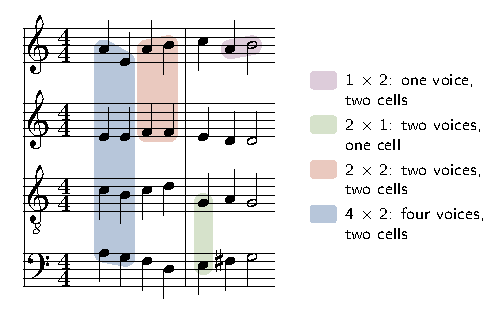
\includegraphics[width=\columnwidth]{hyperedge_shapes}
\caption{A hyperedge of shape $v \times s$ joins $v$ voices over $s$ cells. BWV 40.6, bars 1--2, transposed; one cell per beat for readability, a quarter of a beat in the model.}
\label{fig:shapes}
\end{figure}
\begin{table*}[t]
\renewcommand{\arraystretch}{1.3}
\centering
\caption{Hyperedge shapes, $v$ voices over $s$ cells: what each one is in the music, and the models that use it.}
\label{tab:shapes}
\begin{tabular}{@{}l>{\raggedright\arraybackslash}p{4.0cm}>{\raggedright\arraybackslash}p{9.0cm}@{}}
\hline
Shape & In the music & In the literature \\
\hline
$1 \times 2$ & the move of one voice & pairs of notes of one voice up to four beats apart~\cite{hadjeres2016}; up to 30 notes apart, in a melody~\cite{sakellariou2017} \\
$1 \times 3$, $1 \times 4$ & a figure of one voice & melodic $n$-grams of orders 2 and 3~\cite{witten1993} \\
$2 \times 1$ & the interval between two voices & vertical pairs, and diagonal pairs up to two beats apart~\cite{hadjeres2016} \\
$2 \times 2$ & the motion of two voices & Fux's rules of motion between two parts~\cite{fux1725}; evaluated, not modelled, by Hadjeres et al.~\cite{hadjeres2016} \\
$4 \times 1$ & a sonority & the chord as the hidden state of a hidden Markov model~\cite{allan2004}; the four parts of a slice as one symbol~\cite{whorley2013} \\
$4 \times 2$ & a change of sonority & chord-to-chord transitions, one step per beat~\cite{allan2004}; the interval of each voice to the previous slice~\cite{conklin2002} \\
$4 \times s$, $s \leq 6$ & a progression & $n$-grams of slices up to order 5~\cite{whorley2013} \\
$2 \times 3$, $3 \times 2$, \dots & & none in the sources we checked; measured here \\
\hline
\end{tabular}
\end{table*}

\subsubsection{Shapes in the literature}
Table~\ref{tab:shapes} lists the shapes, what each one is in the music, and the models that use them. Shape $2 \times 2$ is the smallest on which Fux's rules of motion are defined: they forbid reaching a perfect consonance by similar motion, and so forbid parallel fifths and octaves \cite{fux1725}. Pairs of notes miss these rules: in the pairwise model of Hadjeres et al., 61.5\% of the generated $2 \times 2$ configurations occur in the corpus, yet consecutive fifths and octaves are 2 to 10 times more frequent than in the corpus \cite{hadjeres2016}.

\subsubsection{From the corpus to the hypergraph}
The grid turns each voice of a file into a sequence of nodes, one per cell, and every window of $v$ voices and $s$ cells belongs to one class; no window spans a passage that the corpus skips. Each window carries its fold, the position in the bar of its first cell, in Bach the fermata, and for each voice an attack flag that says whether the voice holds its note or attacks a new one, a distinction that Allan and Williams \cite{allan2004} and Whorley et al. \cite{whorley2013} also draw.

\subsubsection{Weights}
The weight of a hyperedge is the support of its class, as in the mining of association rules \cite{agrawal1993}: the share of the windows of its shape that belong to the class, each window counted $1/k$ times for a file with $k$ versions (Section~\ref{sec:transformations}). A class that never occurs has no hyperedge.

\subsubsection{The walk}
The walk moves one walker per voice: at each cell all walkers move together, and a move is more likely when the hyperedges it completes have a higher support. How the supports of overlapping hyperedges combine is still open.

\subsubsection{Which shapes we keep}
A shape stays if a rule of the style is defined on it and if the corpus covers it. We measure every shape up to four voices and four cells, $2 \times 3$ and $3 \times 2$ included. The coverage of a shape is the share of the windows of a held-out fold whose class has a positive support in the other nine folds. We measure it on all windows and on the windows where at least one voice attacks, since held notes are easy to cover. The walk uses the smallest shapes with a rule and a coverage above a threshold fixed before the measures.

\subsection{Transformations}
\label{sec:transformations}

\subsubsection{Transposition}
We move every file to the white keys, so that pieces in different keys add to the same counts. A Bach chorale moves so that its tonic falls on C if its key is major and on A if it is minor, as in BachBot \cite{liang2017}. In Palestrina, a movement in \emph{cantus mollis} moves down a fourth, into \emph{cantus durus}. The shift, the number of semitones that a file moves, is always the nearest one, at most six up or down, so that the voices stay within their range. The transposition is global: a passage that modulates keeps the degrees of the home key, as in Hadjeres et al. \cite{hadjeres2016}, BachBot \cite{liang2017} and BacHMMachine \cite{zhu2021}. Models that follow modulations add the local key as a separate variable: DeepBach as metadata estimated bar by bar \cite{hadjeres2017}, BacHMMachine as a hidden state learned from annotated chorales \cite{zhu2021}. We leave the local key out, because it would give the walk a harmonic analysis and Palestrina's masses have none. The degree is a point of reference, not a constraint: the nodes hold every pitch the corpus uses, so a passage in G keeps its F$\sharp$ and its own classes, measured from C. What the global key loses is sharing. The leading tone that rises to the tonic is one class in C, from B to C, and another in G, from F$\sharp$ to G, each with its own share of the counts; a key that the corpus rarely reaches has few classes. Major and minor chorales are counted together; Hadjeres et al. and Allan and Williams model them apart \cite{hadjeres2016, allan2004}, and counting them apart is an ablation.
% TODO the cost of the global transposition, from notebook 04: next-note bits with the global and the local degree, and the share of new notes off the scale of each.

\subsubsection{Grid}
The model reads time on a grid of equal cells, each a quarter of a beat long: a sixteenth note in Bach and an eighth note in Palestrina (Table~\ref{tab:grid}). Each cell holds the note that sounds at its end, whereas DeepBach \cite{hadjeres2017} takes the note that sounds at its start. The two rules differ only on the nine ornaments of the Bach soprano, where two thirty-second notes share one cell. On all nine, the end rule keeps a note of the chord and drops a note outside it, so it keeps the harmony and loses only the ornament.

\subsubsection{Repeats and versions}
A passage under a repeat sign counts once, as written. Some files write the repeated passage in full instead; when the two occurrences are identical, we skip the second one. Bach has 26 such repeats. Two occurrences that differ by at most 7.4\% of their notes are versions of one passage, and so are two files that differ that little. Each version enters with the weight $1/k$, where $k$ is the number of versions, so that the notes they share count once and each variant counts $1/k$. This is the sequence weighting of Henikoff and Henikoff \cite{henikoff1994}. The threshold of 7.4\% sits in a gap in the data: the closest pair of files above it differs by 10.7\%. With these weights, the corpus that the model counts has 359 rows for 352 Bach chorales, which weigh as 333 pieces, and 1,181 rows for 1,179 Palestrina movements, which weigh as 1,178.

% TODO The measured impact of each transformation on the hypergraph, before and after; why no further transformation applies.
\placeholder{7}

\section{Hypotheses and Methodology}
\label{sec:method}
Every model counted from the corpus is tested on tunes and masses that its counts have not seen.
\subsection{Hypotheses}

% TODO H0 and H1 reworded: the fair test is against Allan and Williams and the count baselines, rebuilt on every fold; DeepBach is a declared reference that has seen the melodies. Directional or not, and why; operational definitions of every measure and threshold; the date on which the hypotheses were fixed.
\placeholder{9}

\subsection{Analytical Approach}

% TODO The walk, its parts and the ablation; the measures, each with its reference; parameters and how they were chosen; software and versions.
\placeholder{10}

\subsection{Validation Approach}

Every number on how well a model counted from the corpus imitates a style comes from cross-validation by group. We split each corpus into ten folds, as Kohavi recommends \cite{kohavi1995}, and test each fold with a model counted on the other nine. A group never crosses a fold, so that the model never meets in training a piece closely related to the one it is tested on. In Bach, a group is a tune, identified by the Zahn number \cite{zahn1889} that When in Rome gives each chorale. Bach set some tunes many times, and a setting of the same tune in training would let the model recall the tune instead of imitating the style. Two chorales also join one group when their top voices contain each other's intervals at 90\% or more, which covers the chorales without an analysis, and so do the versions of one piece. Bach thus has 181 groups, the largest with 13 files on one tune. In Palestrina a group is a mass, so that the movements of one mass never fall on both sides of a split. The corpus holds 101 masses.

We assign the groups to the folds from the largest down, each to the fold with the fewest notes so far. Every fold then holds between 7,784 and 7,909 weighted notes in Bach, and between 67,270 and 70,043 in Palestrina. The assignment has no random part, so every run gives the same folds.

These ten folds are one partition among many, and cross-validation has no unbiased estimate of its own variance \cite{bengio2004}. We therefore repeat the cross-validation on five more assignments of the groups to the folds, drawn at random with fixed seeds, and compare two models only on the same folds. A difference between two models is tested with the t-test for repeated cross-validation, corrected for the overlap of the training sets \cite{nadeau2003, bouckaert2004}. The correction is an approximation: it assumes that the estimates of two folds correlate as much as the size of a test set to the size of a training set.

% TODO The null model, what it preserves and what it randomizes; the test, its statistic, more than 30 null instances, alpha; multiple testing; effect sizes; robustness checks decided in advance.
\placeholder{11}

\section{Results}
\label{sec:results}
% TODO One sentence: the main result, with its number.
\placeholder[1]{12}
\subsection{Data-Driven Analysis}

% TODO Results in the order of the hypotheses, each with its number, null distribution and test outcome; figures with uncertainty; robustness results; null results as results.
\placeholder{13}

\subsection{What can we conclude?}

% TODO For each hypothesis, H0 rejected or not; interpretation and alternative explanations; link to the related work; limitations and threats to validity: internal, construct, external, and the assumptions of the null model.
\placeholder{14}

\section{Conclusions}
\label{sec:conclusions}
% TODO The answer to the research question in two or three sentences; the contributions restated as findings; future work that follows from the limitations. Back matter: data and code availability, references.
\placeholder{15}

\subsection{Data and Code Availability}
\label{sec:availability}
The code is at \url{https://github.com/sclfnc/hypergraph-walks-bach-palestrina}. The data are not redistributed: the notebooks download every source. Both corpora are distributed with music21 \cite{cuthbert2010, cuthbert2026music21}, whose software licence, BSD 3-Clause, does not cover the files of its corpus. The Bach files state no licence, except three \textcopyright{} CCARH (1994). The Palestrina files are \textcopyright{} John Miller (2000). Both of these copyrights reserve the rights to derivative electronic formats. When in Rome \cite{gotham2023, gotham2026wir} is under CC BY-SA 4.0 and the Bach Chorales Melody-Harmony corpus \cite{sears2023} under CC BY 4.0.

\bibliographystyle{IEEEtran}
\bibliography{../references}  % the project's one bibliography, shared with the slides
\end{document}
